\hypertarget{cdefs_8h}{\section{Référence du fichier libc/include/sys/cdefs.h}
\label{cdefs_8h}\index{libc/include/sys/cdefs.\-h@{libc/include/sys/cdefs.\-h}}
}
Ce graphe montre quels fichiers incluent directement ou indirectement ce fichier \-:
\nopagebreak
\begin{figure}[H]
\begin{center}
\leavevmode
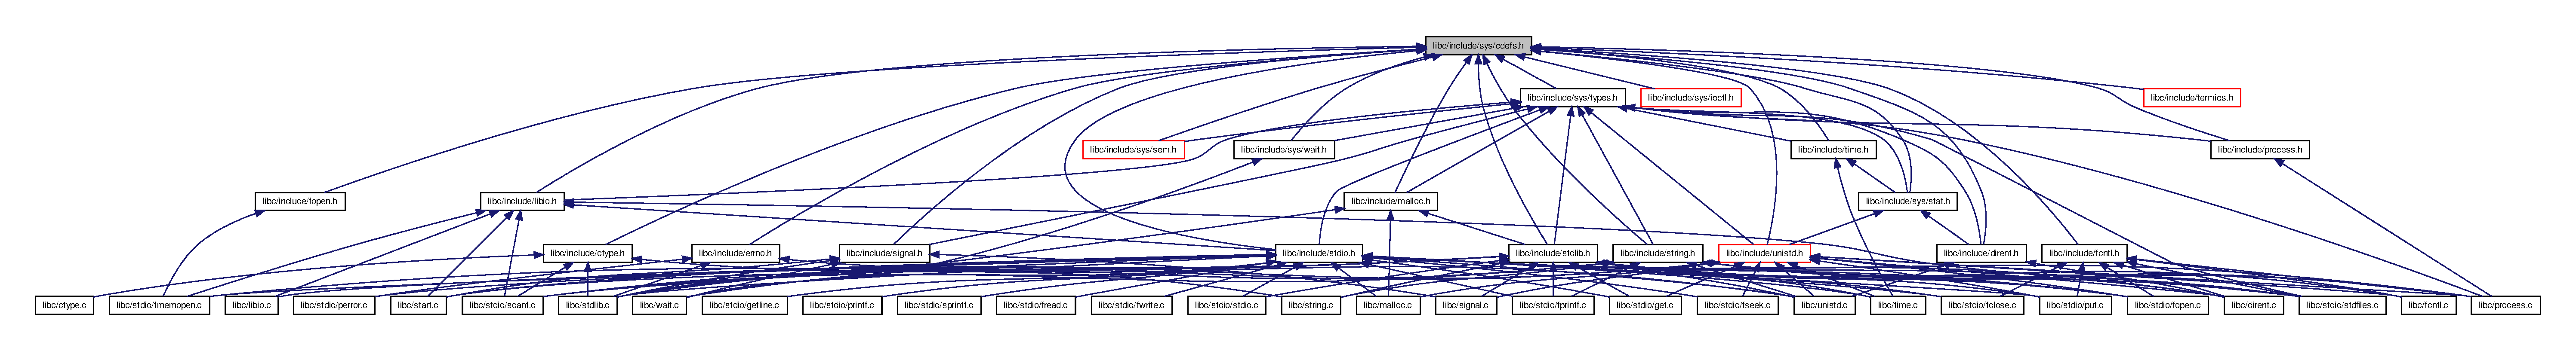
\includegraphics[width=350pt]{cdefs_8h__dep__incl}
\end{center}
\end{figure}


\subsection{Description détaillée}
\begin{DoxyAuthor}{Auteur}
Tac\-O\-S developers
\end{DoxyAuthor}
\hypertarget{wait_8c_LICENSE}{}\subsection{L\-I\-C\-E\-N\-S\-E}\label{wait_8c_LICENSE}
Copyright (C) 2010, 2011, 2012 -\/ Tac\-O\-S developers.

This program is free software; you can redistribute it and/or modify it under the terms of the G\-N\-U General Public License as published by the Free Software Foundation; either version 3 of the License, or (at your option) any later version.

This program is distributed in the hope that it will be useful, but W\-I\-T\-H\-O\-U\-T A\-N\-Y W\-A\-R\-R\-A\-N\-T\-Y; without even the implied warranty of M\-E\-R\-C\-H\-A\-N\-T\-A\-B\-I\-L\-I\-T\-Y or F\-I\-T\-N\-E\-S\-S F\-O\-R A P\-A\-R\-T\-I\-C\-U\-L\-A\-R P\-U\-R\-P\-O\-S\-E. See the G\-N\-U General Public License for more details at \href{http://www.gnu.org/copyleft/gpl.html}{\tt http\-://www.\-gnu.\-org/copyleft/gpl.\-html}

You should have received a copy of the G\-N\-U General Public License along with this program; if not, see \href{http://www.gnu.org/licenses}{\tt http\-://www.\-gnu.\-org/licenses}.\hypertarget{wait_8c_DESCRIPTION}{}\subsection{D\-E\-S\-C\-R\-I\-P\-T\-I\-O\-N}\label{wait_8c_DESCRIPTION}
